\documentclass[12pt]{article}

%nice geometry
\usepackage[a4paper,left=3.5cm, right=3.5cm, top=3cm, bottom=3cm]{geometry}

%if no page numbering needed
\pagestyle{empty}

%figures and html
\usepackage{epsfig}
\usepackage{hyperref}
\usepackage{tikz}

%for author list
\usepackage{authblk}
%configure author list "and" word to spanish
\renewcommand\Authand{ }
\renewcommand\Authands{ }

%for spanish
%\usepackage[spanish]{babel}
%\selectlanguage{spanish}
%\decimalpoint
%\usepackage[latin1]{inputenc}

%add pdfpages
\usepackage[final]{pdfpages}

%to insert watermark
%\usepackage{graphicx}
%\usepackage{type1cm}
%\usepackage{eso-pic}
%\usepackage{color}

%Rename appendix title, as it does not change
%with babel
%\usepackage{appendix}
%\renewcommand{\appendixtocname}{Apéndice}
%\renewcommand{\appendixpagename}{Apéndice}

%change abstract name title
%\addto{\captionsspanish}{\renewcommand{\abstractname}{Abstract}}


\begin{document}

\title{The Large Aperture Gamma Ray Observatory: a Latin American Very Long
Baseline Array of Water Cherenkov Detectors\\Ecuador Site}


%Modelo para incluir dirección electrónica en el pie
% de página
%\author[1]{Author A\thanks{A.A@university.edu}}
%
\author[2]{{ Mario Audelo}}
\author[4]{{ Edgar Carrera}}
\author[4]{{ Dennis Cazar}}
\author[3]{{ Mary D\'{i}az}}
\author[1]{{ Cristina Mantilla}}
\author[1]{{ and Nicol\'{a}s V\'{a}squez}}
%\author[ ]{{\\\it for the LAGO Collaboration}}
\affil[1]{Escuela Polit\'{e}cnica Nacional, Quito-Ecuador}
\affil[2]{Escuela Superior Polit\'{e}cnica del Chimborazo, Riobamba-Ecuador}
\affil[3]{Universidade Estadual de Campinas, Campinas-Brazil}
\affil[4]{Universidad San Francisco de Quito, Quito-Ecuador}


%\date
%inicio del documento

\maketitle

\begin{abstract}
This article describes the design and construction of the WCD detector prototype that has been implemented in Ecuador as part of the LAGO Collaboration array. Some details about the current status of the detector are also given, as well as some first histograms obtained with the collected data. Finally we report new locations and sites under planification.
\end{abstract}

\section{Detector Prototype}

We use a commercial water tank, with a capacity of about ${1100\ {\rm l}}$, and low cost accessories to build the detector system.  From bottom to top, the tank is mostly cylindrical, followed by a truncated-cone section and a cylindrical end at the top. The radius of the base of the main cylinder is $55\ {\rm cm}$, and its height $110\ {\rm cm}$.  The truncated cone section base matches that of the main cylinder and has an apothem of $32\ {\rm cm}$. The upper cylindrical part, which hosts the water tank cap, has a diameter of $50\ {\rm cm}$ and a height of $11\ {\rm cm}$. A detailed drawing can be seen in Figure~\ref{fig:tank}.

\begin{figure}[!ht]
  \centering
 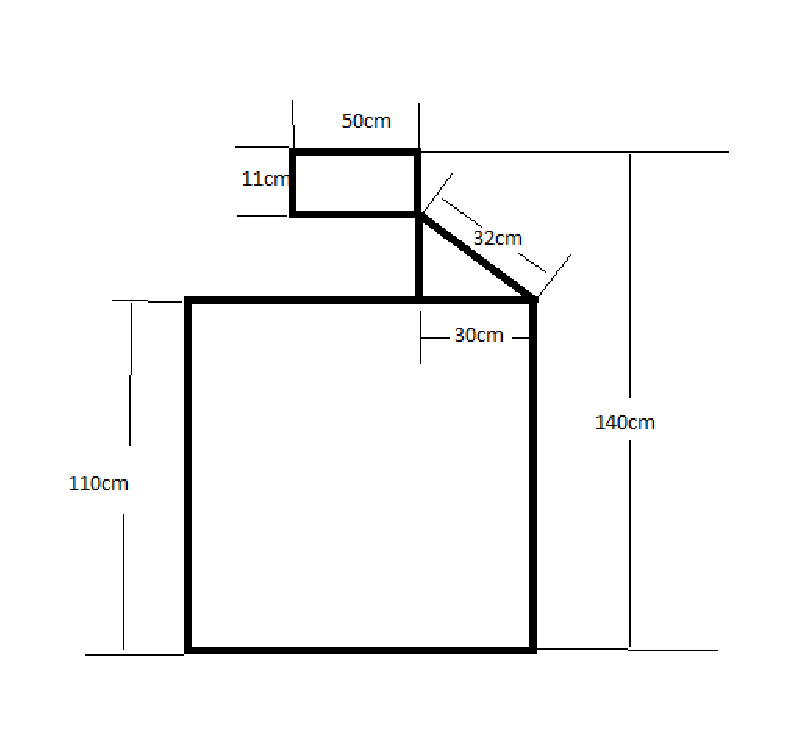
\includegraphics[width=0.45\textwidth]{chimbito_dimensiones.eps}
  \caption{Dimensions of the Cherenkov water tank prototype.}
  \label{fig:tank}
 \end{figure}

The external walls of the tank are protected with four layers of
high-density nonreflective black polyethylene. To guarantee good
reflectivity and diffusivity, the internal walls of the tank are lined with
Banner-type material. We also use ${{\rm Tyvek^{\tiny \textregistered}}}$
as inner lining material supported by a frame inside the tank and floating
on top of the water. A photomultiplier tube (PMT) Photonis XP$1802$ $9$'',
is mounted for Cherenkov light collection and is placed at the top and
central part of the detector cap. A hole was cut on the ${{\rm Tyvek^{\tiny
      \textregistered}}}$ surface in order for the PMT to protrude into the inner part of the tank. The PMT is connected to a digitizer board and a FPGA, whose connection was developed at the ``Laboratorio de detecci\'on de part\'iculas y radiaci\'on (DPR)'' Bariloche, Argentina. The prototype is shown in Figure~\ref{fig:detector}. Special care has been taken to isolate this device and its electronics board from moisture and to avoid water entering the PMT hose. 

\begin{figure}[!ht]
  \centering
 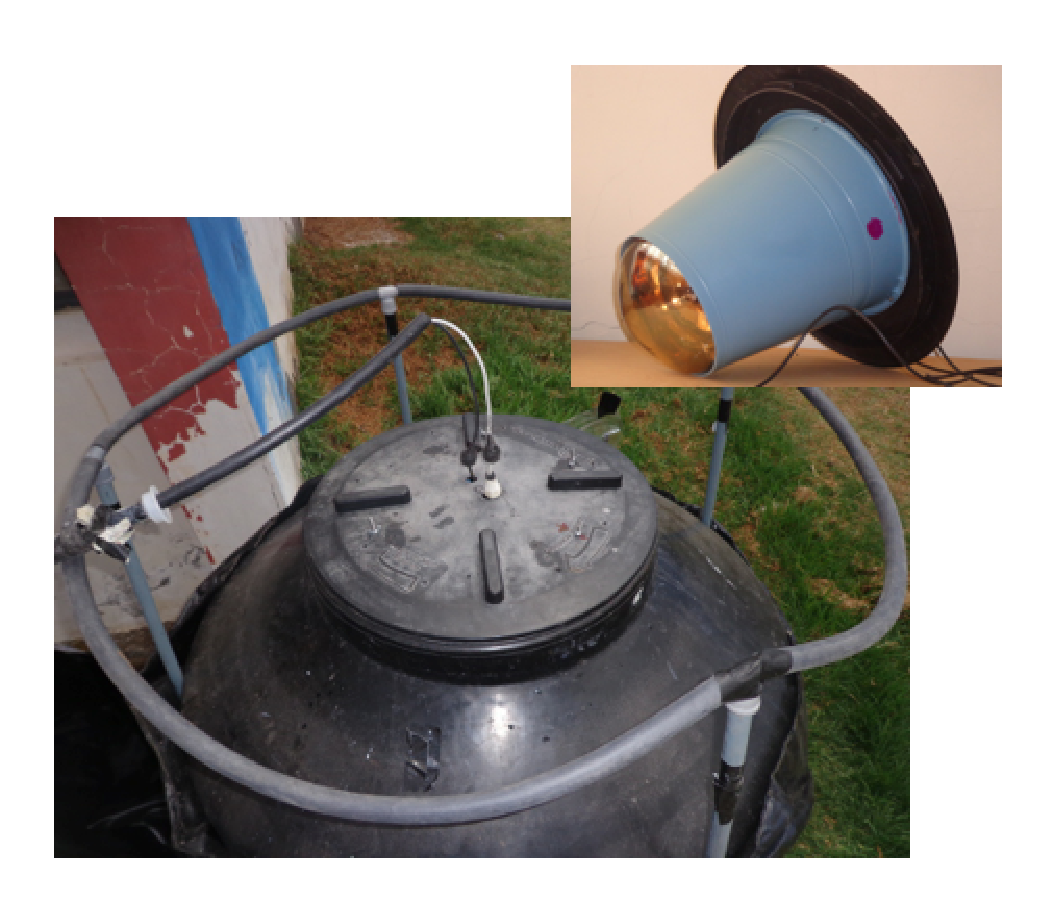
\includegraphics[width=0.45\textwidth]{icrc2013-1208-01.eps}
  \caption{Water Cherenkov Detector prototype ``Chimbito'' installed at Riobamba, Ecuador (2784 m a.s.l.). The PMT and its support are shown in the inset.}
  \label{fig:detector}
 \end{figure}

The PMT works at a spectral range from $270$ to $650$~nm, with a maximum sensitivity at around $420$~nm. It is practically noiseless and can amplify photons as much as ${160\ {\rm dB}}$.

The PMT is connected to one of the three channels of the data acquisition system. A digitizer board filters and amplifies 
the signal prior to the Analog to Digital Conversion (ADC), performed at a rate of ${40\ {\rm MSPS}}$ with a $10$-bits word using ${{\rm AD}9203}$ ${\rm ADC}$ from Analog Devices. The digital signals are processed by a Digilent NEXYS-$2$ FPGA board, which contains the software needed to acquire and process the digitized pulses from the PMT. 

In order to implement data corrections, due to pressure and temperature variations, a HP$03$S pressure and temperature sensor is connected to the NEXYS-$2$ FPGA. Also, a GPS module Motorola GT Plus is connected to the NEXYS-2 in order to provide a PPS (Pulse Per Second) signal for the time synchronization of the data. Finally, the data is collected via a serial line by an acquisition PC, and stored for further analysis.

With these characteristics the data acquisition system is capable of obtaining 3 channel pulses every $25$~ns. The NEXYS-$2$ FPGA board is always recording data in two buffers, but this information is transferred to the PC only if the pulse is higher than a threshold; a different trigger threshold value can be set for each channel. In this way, whenever a pulse triggers, a full trace of the $3$ channels is sent, containing $12$ data strings: $2$ pre-trigger bins, the trigger bin and $9$ post-trigger bins. Furthermore, a time\-stamp of the trigger pulse and a trigger counter are also added. The data can be read at about $10000$ pulses per second.

In order to allow operation at higher rates (for large detectors, high altitude and/or low geomagnetic cutoff), a sub-trigger mode is available where only the highest value of the triggering pulse is transferred, together with the trigger timestamp. This mode allows to record up to $150000$ pulses per second. Every second, a block of extra data containing the real time, clock performance, temperature and pressure sensor information is added to the data flow. A data file per hour is stored and compressed in the host PC. At normal operation, the WCD detector would produce tens of GB per day.

The shock chlorination technique has been used to improve the quality and purity of the stored water. This process consists of the dilution of a high concentration of chlorine ${\rm  Cl_{2}}$ into the water (approximately 150 mg of ${\rm Cl_{2}}$ per liter) in order to purify it. This method allows very low light absorbance in a spectral range from $350$ to $750$~nm. However, due to its low cost and relatively easy way to apply, it has been chosen as the default method of purification. It is important to mention that it is the first time that this process is used to purify water for WCD in the LAGO Collaboration. Furthermore, amino-G, ${\rm NH_{2}C_{10}H_{5}(SO_{3}H)S)_{3}Na}$, the most common wavelength shifter used in water Cherenkov detectors, has been added to the water in a concentration of $1$~mg per liter. Studies report that, with this addition, the efficiency of the detector increases by a factor of $3$ without loosing the directionality of Cherenkov light~\cite{Badino:1981ps}.

\section{Description of the Location and Operational Status of the Detector}

The WCD prototype ``Chimbito'' was installed in August $2012$ at Escuela Polit\'{e}cnica del Chimborazo (ESPOCH) at $2870$~m a.s.l, which is about $60\ {\rm km}$ from the Chimborazo volcano. The campus sits at a latitude of ${1^{\circ}\  39'\ 58''\ {\rm S}}$ and a longitude of ${78^{\circ}\  39'\ 33''\ {\rm O}}$. Based on reference~\cite{rigidity} the rigidity cut-off at these coordinates is about ${15.02\ {\rm GeV}}$.

The detector took initial data for two consecutive months in 2012 before its PMT started to fail, most likely due to moisture inside. Data taking restarted in July 2013, and has been stable ever since. Figure ~\ref{fig:pulse} shows an individual pulse and the mean signal response of the detector for data taken in September 2013.

 \begin{figure}[!ht]
  \centering
 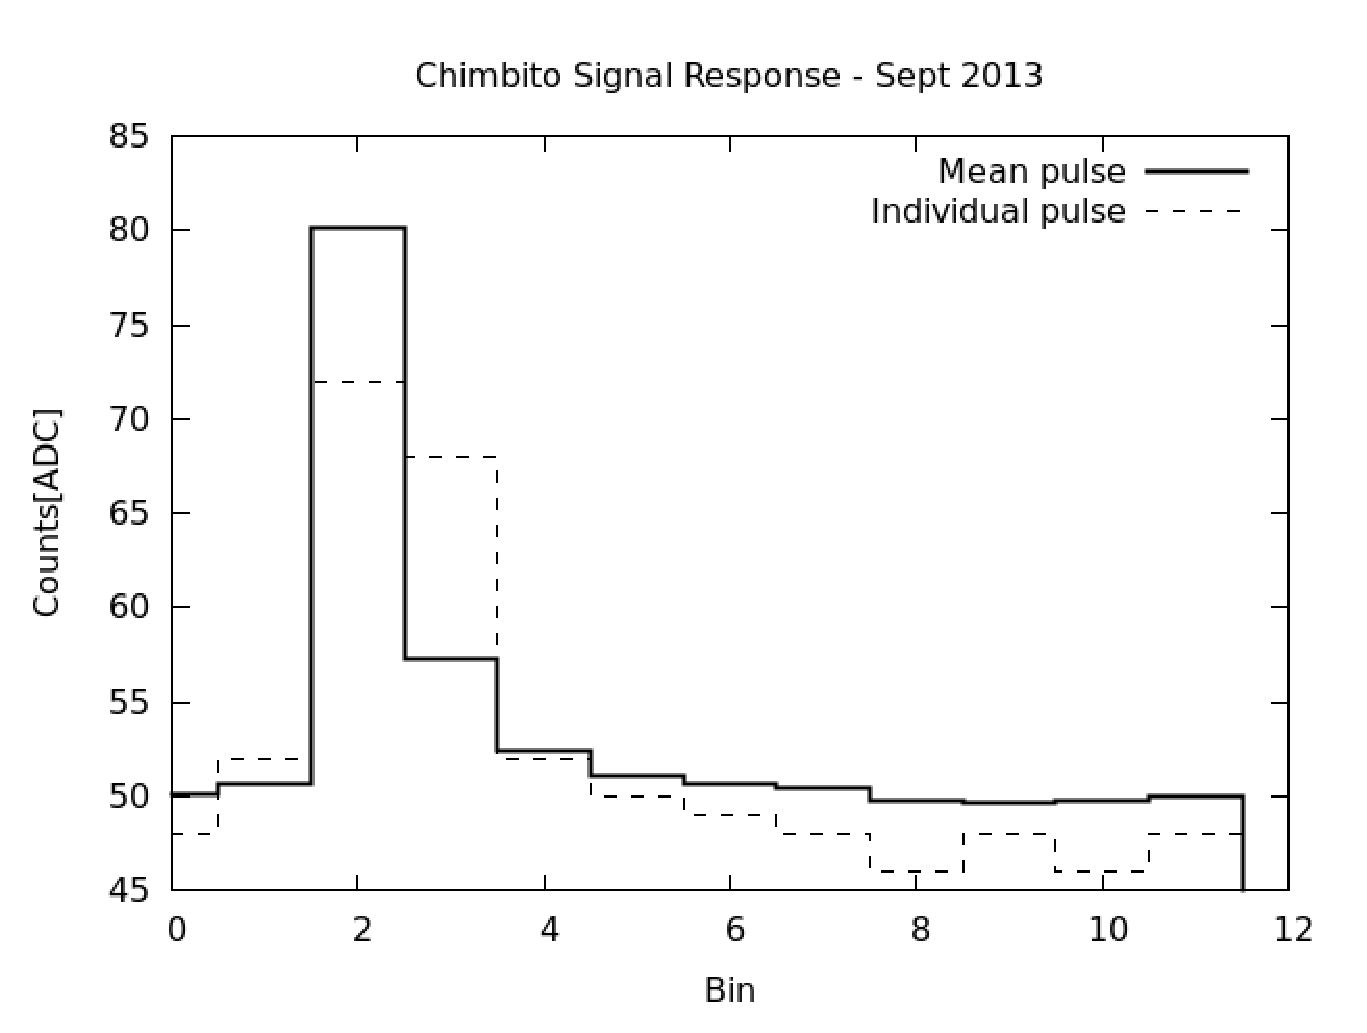
\includegraphics[width=0.8\textwidth]{promedioSep21h.eps}
  \caption{Mean signal response ``Chimbito'' September 2013. The individual signal response of a pulse is also shown.}
  \label{fig:pulse}
 \end{figure}

Calibration histograms have been extracted from the collected data. A total charge histogram and a peak histogram for data collected between July and November of $2013$ are shown in Figure~\ref{fig:charge} and Figure~\ref{fig:peak} respectively. It is evident from these and other first plots obtained that some adjustments need to be done to the detector in order to find an optimal operation point and improve its performance. 

 \begin{figure}[!ht]
  \centering
 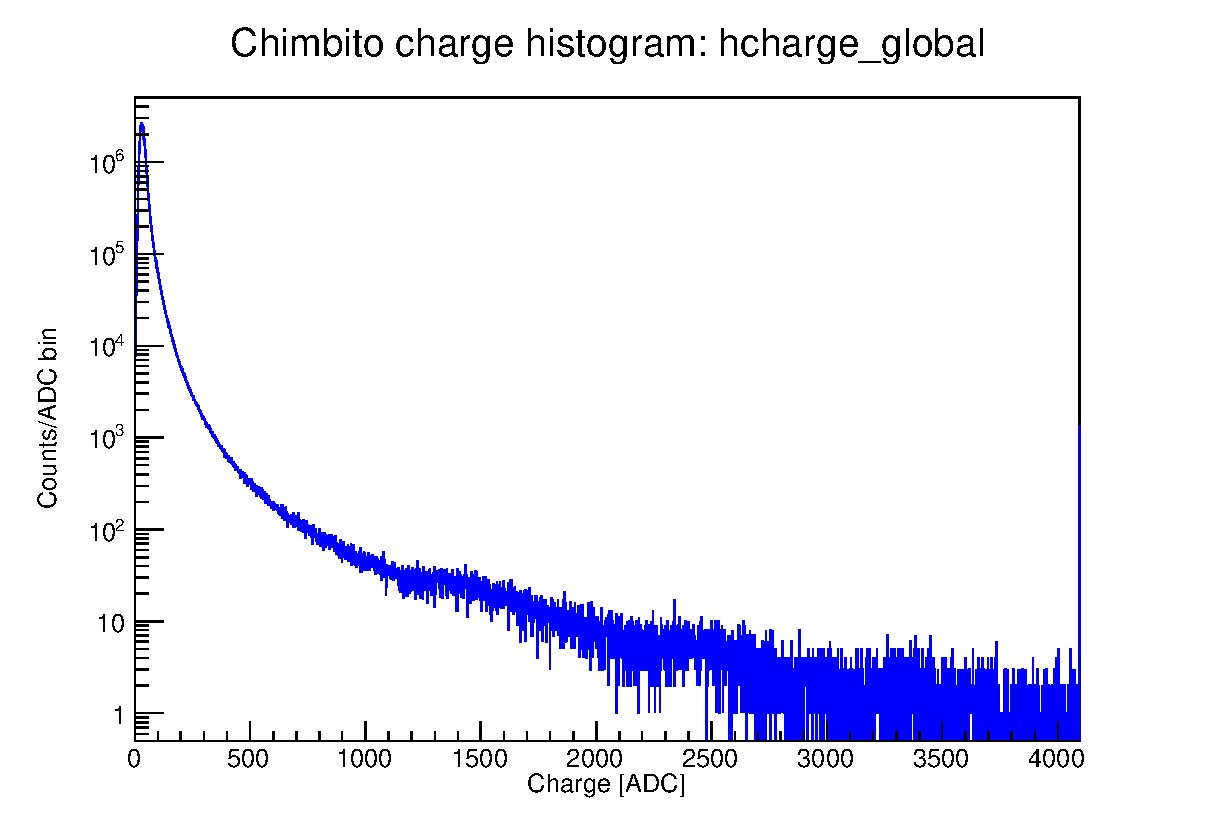
\includegraphics[width=0.8\textwidth]{charge_histo_chimbito_jul_nov_2013.eps}
  \caption{Charge histogram with data taken between July and November 2013.}
  \label{fig:charge}
 \end{figure}
 
  \begin{figure}[!ht]
  \centering
 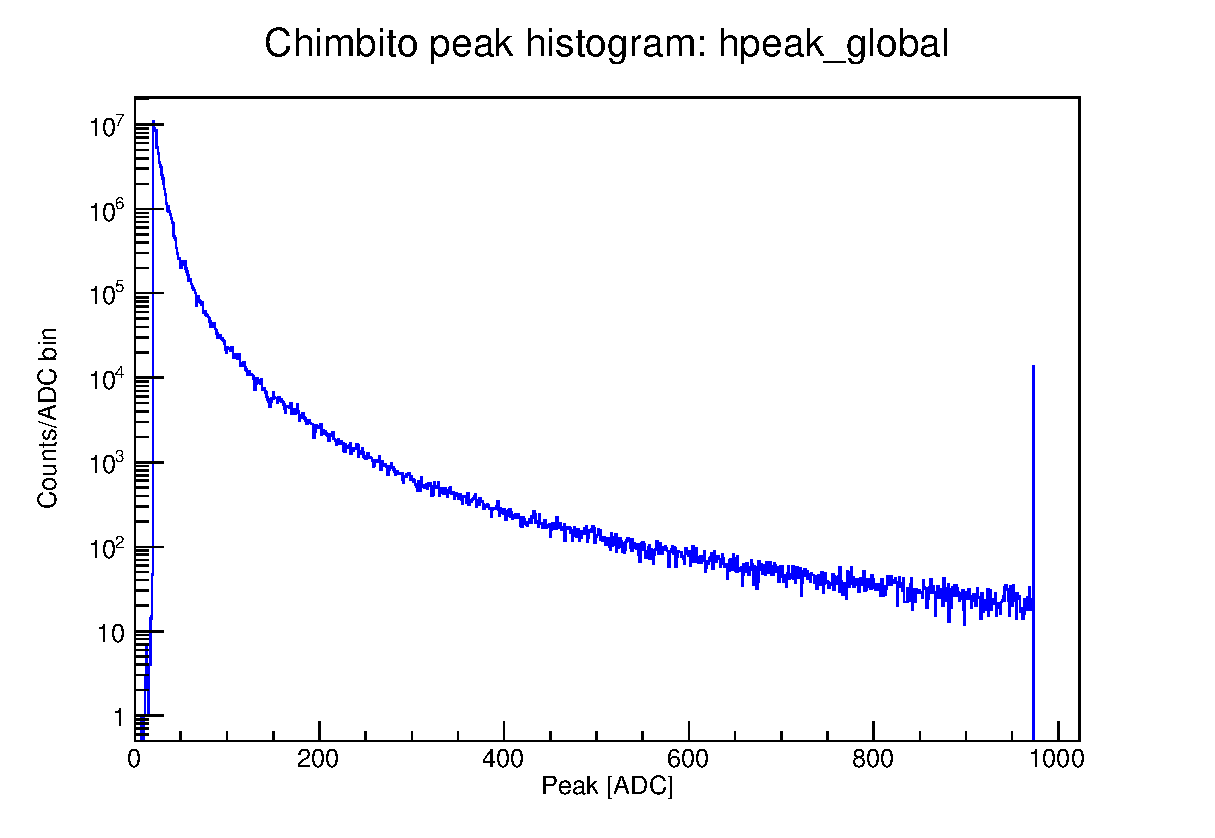
\includegraphics[width=0.8\textwidth]{peak_histo_chimbito_jul_nov_2013.eps}
  \caption{Peak histogram with data taken between July and November 2013.}
  \label{fig:peak}
 \end{figure}
 
Currently, all the flowing data is being analyzed and interpreted in order to assess the true status of the detector, and to identify any possible changes to the hardware configuration. The calibration of the detector using the muon peak is expected to be done in a short time.

In the near future, the final objective is to locate a new detector in the
Chimborazo snowcap foothills at $4800$~m a.s.l., which will be, to our
knowledge, the second highest LAGO site after Chacaltaya ($5300$~m a.s.l.),
Bolivia. The data taken from this new detector is expected to be compared
with the data obtained with the ``Chimbito'' detector. Due to the high altitude of this site  this comparison could increase the detection sensitivity of transient events emitting high energy photons.

As a final note, it is worth mentioning that a new WCD prototype
``Panchito'' is under construction at Cumbaya, Quito ($2398$~m a.s.l.),
Ecuador. This detector will be located at Universidad San Francisco de
Quito (USFQ). We will use a commercial water tank of ${2500\ {\rm l}}$
similar to the one used in ``Chimbito'' design but with a geometry better
suited for photon detection. The radius of the base of the main cylinder is
$78.4\ {\rm cm}$, and its height $146\ {\rm cm}$. The upper cylindrical cap
has a diameter of $55\ {\rm cm}$. The internal walls of the WCD will be
covered by ${{\rm Tyvek^{\tiny \textregistered}}}$ and Banner-type material
in a manner similar to the detector in Riobamba. The PMT XP$1802$ $9$''produced by Photonis will be connected to an acquisition board. It has sensitivity over a wide spectral range, from $270$ to $650$~nm, and can amplify photons as much as ${160\ {\rm dB}}$. The performance of the PMT and the electronics has been verified. The prototype electronics share similar characteristics with ``Chimbito'' WCD and will be installed in the detector in February 2014.

A new high altitude site near the east side of Pichincha Volcano, Cruz Loma at $4100$~m a.s.l., is under consideration. This detector is expected to be used for high energy physics analysis. Meanwhile, ``Chimbito'' and ``Panchito'' detectors will be used for solar physics analysis and software development. Multiple comparisons could be done using the data obtained with this detector array.

\begin{thebibliography}{}
\bibitem{Badino:1981ps} G. Badino, P. Galeotti, L. Periale, O. Saavedra and A. Turtelli, \emph{Nucl. Instrum. Meth.}, 185, 587, 1981.

\bibitem{rigidity} Nymmik, R.A. and Panasyuk, M.I. and Petrukhin, V.V. and Yushkov, B.Yu., \emph{Cosmic Research}, 47, 3, 191-197, 2009.
\end{thebibliography}
\end{document}
